\documentclass[12pt]{article}
\usepackage{fullpage,enumitem,amsmath,amssymb,graphicx}
\usepackage{graphicx} % This is a package for including graphics in your solution.
\usepackage{listings}
\usepackage[final]{pdfpages}

\begin{document}

\begin{center}
{\Large CS168 Spring Assignment 2}

\begin{tabular}{rl}
SUNet ID(s): 05794739 & \\
Name(s): & Luis A. Perez \\
Collaborators: &
\end{tabular}
\end{center}

By turning in this assignment, I agree by the Stanford honor code and declare
that all of this is my own work.

\section*{Part 1}

\begin{enumerate}[label=(\alph*)]
  \item
    \begin{verbatim}
import collections
import matplotlib.pyplot as plt
import scipy

import numpy as np
import pandas as pd
import seaborn as sns
import os
import warnings

from typing import Dict, List, Text, Tuple

# Make figure larger
plt.rcParams['figure.figsize'] = [10, 5]

class Globals:
    """Class holding globals to avoid polluting workspace."""
    DATA_DIR: Text = 'p2_data'
    LABEL: Text = 'label.csv'
    GROUPS: Text = 'groups.csv'
    DATA: Text = 'data50.csv'

def makeHeatMap(data, names, color, outputFileName):
    """Makes a 20x20 heatmap from the given 20x20 data matrix."""
    # to catch "falling back to Agg" warning
    with warnings.catch_warnings():
        warnings.simplefilter("ignore")
        # code source: http://stackoverflow.com/questions/14391959/heatmap-in-matplotlib-with-pcolor
        fig, ax = plt.subplots()
        # create the map w/ color bar legend
        heatmap = ax.pcolor(data, cmap=color)
        cbar = plt.colorbar(heatmap)

        # put the major ticks at the middle of each cell
        ax.set_xticks(np.arange(data.shape[0]) + 0.5, minor=False)
        ax.set_yticks(np.arange(data.shape[1]) + 0.5, minor=False)

        # want a more natural, table-like display
        ax.invert_yaxis()
        ax.xaxis.tick_top()

        ax.set_xticklabels(range(1, 21))
        ax.set_yticklabels(names)

        plt.tight_layout()

        plt.savefig(outputFileName, format='png')
        plt.close()

def read_data() -> Tuple[Dict[int, int], Dict[int, List[int]], pd.DataFrame]:
    """Reads the relevant data files.
    
    Returns:
        A tuple of items. The bag of words object and for each 
        article (keyed by articleId) and a mapping from
        groupId to a list of corresponding articleIds in that group.
        Also the entire dataset as a pd.DataFrame.
    """
    # Maps to groupId.
    labels = pd.read_csv(
        os.path.join(Globals.DATA_DIR, Globals.LABEL), header=None,
        names=['groupId'])
    labels['articleId'] = range(1, len(labels) + 1)
    # Maps to groupName.
    groups = pd.read_csv(
        os.path.join(Globals.DATA_DIR,
                     Globals.GROUPS), header=None,
        names=['name'])
    groups['groupId'] = range(1, len(groups) + 1)
    data = pd.read_csv(
        os.path.join(Globals.DATA_DIR, Globals.DATA), header=None,
        names=['articleId', 'wordId', 'count'])
    data = data.merge(labels, on='articleId').merge(groups, on='groupId')
    
    numArticles = max(data.articleId)
    numWords = max(data.wordId)
    # Load into a sparse matrix of (numArticles x numWords)
    sparse_data = np.array(data['count'])
    row_idx = np.array(data['articleId']) - 1
    col_idx = np.array(data['wordId']) - 1
    sparse_matrix = scipy.sparse.csr_matrix((sparse_data, (row_idx, col_idx)), shape=(numArticles, numWords))
    
    # Transform into a dictionary mapping articleId to a collections.Counter
    # object counting each word (based on wordId).
    group_to_name = {groupId : data[data.groupId == groupId].name.iloc[0]
                    for groupId in data.groupId.unique()}
    article_to_group = {articleId : data[data.articleId == articleId].groupId.iloc[0]
            for articleId in data.articleId.unique()}
    group_to_article = { groupId : data[data.groupId == groupId].articleId.unique()
                       for groupId in data.groupId.unique()}
    return sparse_matrix, group_to_article, group_to_name, article_to_group

def l2_dist(X, Y):
    """Computes the L2 pairwise distance between all elements in X,Y.
    
    Args:
        X: An (n,k) matrix where each row is an element.
        Y: An (m,k) matrix where each row is an element.
        
    Returns:
        D: An (n,m) matrix where D[i][j] is the distance L2 distance
            between X[i,:] and Y[j,:].
    """
    (n,k1), (m, k2) = np.shape(X), np.shape(Y)
    assert k1 == k2
    k = k1
    X2 = np.diag(np.dot(X, X.T).todense()).reshape((n, 1))
    Y2 = np.diag(np.dot(Y, Y.T).todense()).reshape((1, m))
    XY = np.dot(X, Y.T)
    return -np.sqrt(X2 + Y2 - 2*XY)

def cosine_dist(X, Y):
    """Computes the cosine pairwise distance between all elements in X,Y.
    
    Args:
        X: An (n,k) matrix where each row is an element.
        Y: An (m,k) matrix where each row is an element.
        
    Returns:
        D: An (n,m) matrix where D[i][j] is the distance L2 distance
            between X[i,:] and Y[j,:].
    """
    (n,k1), (m, k2) = np.shape(X), np.shape(Y)
    assert k1 == k2
    k = k1
    Xnorm = np.sqrt(np.diag(np.dot(X, X.T).todense()).reshape((n, 1)))
    Ynorm = np.sqrt(np.diag(np.dot(Y, Y.T).todense()).reshape((1, m)))
    XY = np.dot(X, Y.T)
    return XY / np.multiply(Xnorm, Ynorm)

def jaccard_dist(X, Y):
    """Computes the Jaccard pairwise distance between all elements in X,Y.
    
    Args:
        X: An (n,k) matrix where each row is an element.
        Y: An (m,k) matrix where each row is an element.
        
    Returns:
        D: An (n,m) matrix where D[i][j] is the distance L2 distance
            between X[i,:] and Y[j,:].
    """
    (n,k1), (m, k2) = np.shape(X), np.shape(Y)
    assert k1 == k2
    k = k1
    
    def ones_on_col(i):
        row_ind = [k for k in range(n)]
        col_ind = [i for _ in range(m)]
        data = np.ones(m)
        return scipy.sparse.csr_matrix((data, (row_ind, col_ind)), shape=(n, n))
    
    # Duplicate X to be [X, X, X, ... X] m times (so just stack them).
    stackedX = scipy.sparse.vstack(X for _ in range(m))
    # Duplicate the rows if Y each n times.
    duplicatedY = np.dot(scipy.sparse.vstack(ones_on_col(row) for row in range(m)), Y)
    mins = stackedX.minimum(duplicatedY) # (n x m) x k
    maxs = stackedX.maximum(duplicatedY) # (n x m) x k
    minSums = np.sum(mins, axis=1).reshape((n,m))
    maxSums = np.sum(maxs, axis=1).reshape((n,m))
    return (minSums / maxSums)

def average_similarity(distances, groupA, groupB) -> float:
    """Computes the average similarity between the two specified groups.
    
    Args:
        distances: A distance matrix computing all distances between all articles.
        groupA: A list of articleIdx belong to groupA.
        groupB: A list of articleIdx belong to groupB.
    
    Returns:
        The average of the similarities between all pairings in A and B.
    """
    # Even though all of our existing sim_fn are symmetric, do
    # all pairs in-case this doesn't hold true in general.
    scores = [distances[Aidx - 1, Bidx - 1]
              for Aidx in groupA for Bidx in groupB]
    return np.mean(scores)

def get_similarity_matrix(db, groups_to_articles, sim_fn, max_groups=None):
    """Computes the similarity matrix using the given sim_fn for all groups.
    
    Args:
        db: Sparse matrix where each row is an article.
        groups_to_articles: Mapping from groupIdx to a list of articleIdx belong to that group.
        sim_fn: Similarity function to use.
    
    Returns:
        A 20x20 matrix with the average similarity between all pairs of groups.
    """
    groups = sorted(groups_to_articles.keys())
    # Similarity between all pairs of articles.
    D = sim_fn(db, db)
    data = np.zeros((20,20))
    for i, groupA in enumerate(groups):
        for j, groupB in enumerate(groups):
            data[i][j] = average_similarity(
                D, groups_to_articles[groupA], groups_to_articles[groupB])
    return data

def get_all_sim_matrices(articles, groups_to_articles, sim_fns):
    """Computes all similarity matrices for all given sim_fns."""
    data = {}
    for name, sim_fn in sim_fns.items():
        data[name] = get_similarity_matrix(articles, groups_to_articles, sim_fn)
    return data

def plot_heatmaps(input_data, sim_fns):
    """Plots and saves heatmaps for different similarity functions."""
    articles, groups_to_articles, group_names, _ = input_data
    names = [group_names[i] for i in sorted(group_names.keys())]
    all_data = get_all_sim_matrices(articles, groups_to_articles, sim_fns)
    for name, data in all_data.items():
        makeHeatMap(data, names, color='Blues',
                    outputFileName="figures/{name}.png".format(name=name))

def problem_1b():
    """Solves problem 2b from Mini-Project 2"""
    input_data = read_data()
    plot_heatmaps(input_data, {
        'Cosine' : cosine_dist,
        'Jaccard': jaccard_dist,
        'L2' : l2_dist })

problem_1b()
    \end{verbatim}
  \item
    We now show the heat maps for each of the above strategies.

    \begin{figure}[!ht]
      \centering
      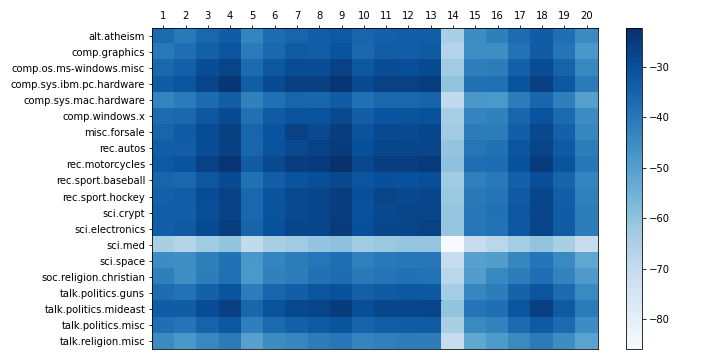
\includegraphics[scale=0.5]{figures/L2.png}
      \caption{$L_2$ Similarity Metric Heat Map.}
      \label{fig:l2}
    \end{figure}
    \begin{figure}[!ht]
      \centering
      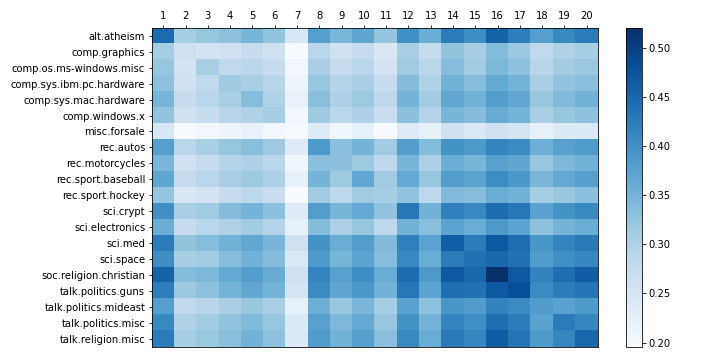
\includegraphics[scale=0.5]{figures/Cosine.png}
      \caption{Cosine Similarity Metric Heat Map.}
      \label{fig:cosine}
    \end{figure}
    \begin{figure}[!ht]
      \centering
      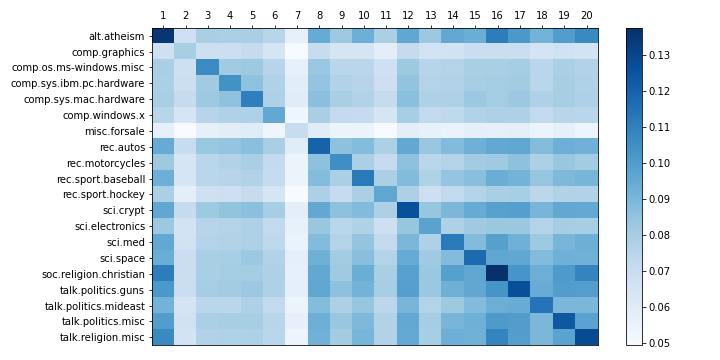
\includegraphics[scale=0.5]{figures/Jaccard.png}
      \caption{Jaccard Similarity Metric Heat Map.}
      \label{fig:jaccard}
    \end{figure}

  \item 
    Based on the heat maps, it appears that the most reasonable similarity metric is the Jaccard Similarity Metric (see Figure \ref{fig:jaccard}). This metric works well for our particularly datasets due to the sparsity of the vectors representing each document, which means the presense of zero values won't overwhelm the metric (as is the case with the $L_2$ norm metric). Since we only look at words that occur in the two documents, the metric is a reasonable approximation for how much ``overlap'' (measured in the number of words intersecting) occurs between two documents.

    Similarly, the cosine similarity metric appears to also be a decent metric for our datasets (see Figure \ref{fig:cosine}). The most likely reason for this is that two documents are highly similar if the angle $\theta$ made between the two vectors is small (so the documents are pointing in the same direction). Since the basis we use corresponds to a count of words, documents which point in similar directions will simply correspond to documents whose word counts for each word are similar. 
\end{enumerate}

\newpage
\section*{Part 2}

\begin{enumerate}[label=(\alph*)]
  \item
    The code used to generate the heatmap in Figure \ref{fig:classification} is given below. This code is used in addition to the helper functions from Part 1.

    The classification accuracy is 45.6\%. 
\begin{verbatim}
def find_nearest_neighbor(database, sim_fn):
    """Finds the nearest neighbor document in the database to all other documents.
    
    Args:
        database: Sparse matrix with all possible articles.
        sim_fn: The similarity functions to use.
    
    Returns:
        The articleIdx corresponding to the nearest neighbors.
    """
    D = sim_fn(database, database) # (n, n)
    (n, _) = D.shape
    # Ignore self-similarity by making it smaller than everything else.
    D = D - 10*(D.max() * np.identity(n))
    # Take the argmin to get the article indeces. +1 to move to articleIdx space.
    return np.array(D.argmax(axis=0)).flatten() + 1

def classification_count(groupA, neighbor_group, groupBId):
    """Counts the number of articles in groupA whose nearest neighbor is in groupB."""
    return len([1 for articleId in groupA
                if neighbor_group[articleId] == groupBId])

def get_classification_matrix(db, groups_to_articles, article_to_groups, sim_fn):
    """Computes the similarity matrix using the given sim_fn for all groups."""
    # array[i - 1] gives articleIdx of nearest neighbor.
    article_to_neighbor = find_nearest_neighbor(db, sim_fn)
    neighbor_group = { articleId : article_to_groups[article_to_neighbor[articleId - 1]]
                      for articleId in article_to_groups }
    data = np.zeros((20, 20))
    groups = sorted(groups_to_articles.keys())
    for i, groupA in enumerate(groups):
        for j, groupB in enumerate(groups):
            data[i][j] = classification_count(
                groups_to_articles[groupA], neighbor_group, groupB)
    return data

def problem2a():
    db, groups_to_articles, group_names, article_to_group = read_data()
    data = get_classification_matrix(db, groups_to_articles, article_to_group, cosine_dist)
    names = [group_names[i] for i in sorted(group_names.keys())]
    makeHeatMap(data, names, color='Blues',
                    outputFileName="figures/classification.png")

problem2a()
\end{verbatim}

    \begin{figure}[!ht]
      \centering
      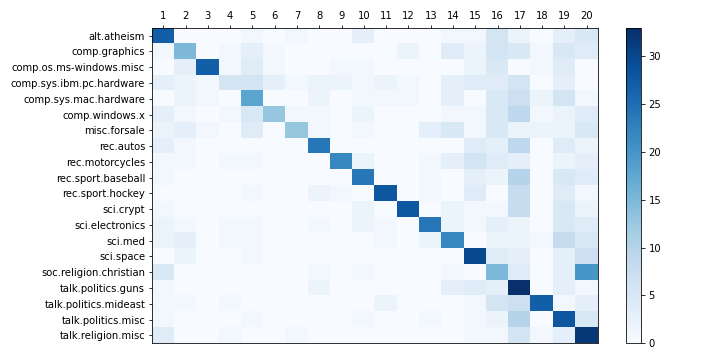
\includegraphics[scale=0.5]{figures/classification.png}
      \caption{Classification Accuracy. Each square (A,B) is a count of the number of articles in A whose nearest neigbor is in group B}.
      \label{fig:classification}
    \end{figure}

  \item
    The matrix is (a) is not symmetric because the metric used is not symetric. While in 1(b) our similarity metrics where symetric (that is to say, the similarity between $A$ and $B$ is the same as the similarity between $B$ and $A$), this is not the case for (a).

    To be concrete, the nearest neighbor measure is not symetric. If $A$'s nearest neighbor is $B$, this does not imply that $B$'s nearest neighbor is $A$. For a trivial example, consider three points on the number line $\{A =0, B=10, C=11\}$. While $A$'s nearest neighbor is $B$, $B$'s nearest neighbor is $C$.

  \item
    The code used to generate Figures \ref{fig:classification_d_10}, \ref{fig:classification_d_25}, \ref{fig:classification_d_50}, and \ref{fig:classification_d_100} is presented below.

    The accuracy for each setting is:

      Classification accuracy: 13.80\% for classification with $d=10$.

      Classification accuracy: 23.10\% for classification with $d=25$.
      
      Classification accuracy: 32.00\% for classification with $d=50$.
      
      Classification accuracy: 38.00\% for classification with $d=100$.

      The only value that is somewhat comparable is $d =100$, which achieves an accuracy close to the full similarity matching, at a much cheaper cost. This is confirmed by the corresponding heatmap (see Figure \ref{fig:classification_d_100}).

\begin{verbatim}
def random_projection(db, d: int):
    (n, k) = db.shape
    M = scipy.sparse.csr_matrix(np.random.normal(size=(d, k)))
    return np.dot(db, M.T) # (n, d)

def problem2c():
    db, groups_to_articles, group_names, article_to_group = read_data()
    
    for d in [10, 25, 50, 100]:
        projected = random_projection(db, d)
        plotHeatMaps2(projected, groups_to_articles,
                      group_names, article_to_group, figName="classification_d=%s" % d,
                      nearest_neigbor_fn=find_nearest_neighbor)

problem2c()
\end{verbatim}
    
    The generated figures are:
    \begin{figure}[!ht]
      \centering
      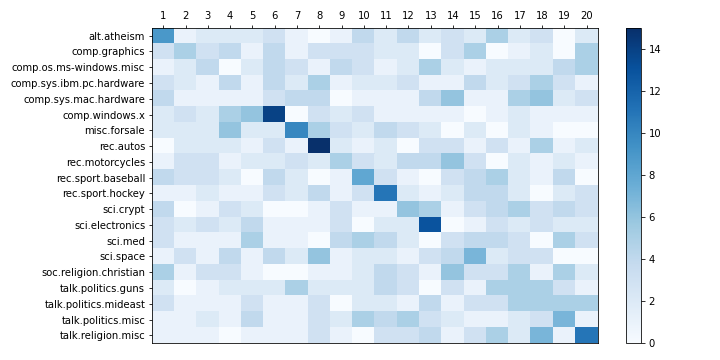
\includegraphics[scale=0.5]{figures/classification_d=10.png}
      \caption{Classification Accuracy. Each square (A,B) is a count of the number of articles in A whose nearest neigbor is in group B. This is for $d=10$}
      \label{fig:classification_d_10}
    \end{figure}
    \begin{figure}[!ht]
      \centering
      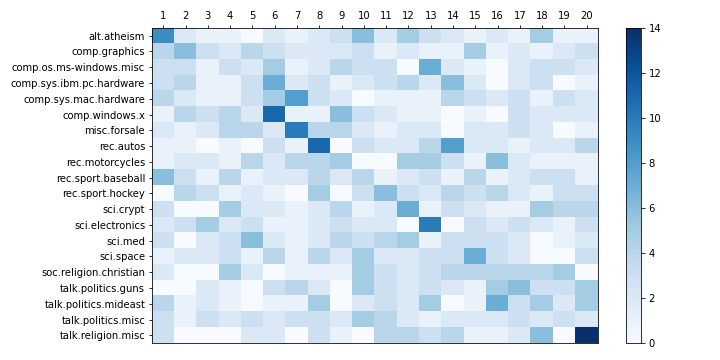
\includegraphics[scale=0.5]{figures/classification_d=25.png}
      \caption{Classification Accuracy. Each square (A,B) is a count of the number of articles in A whose nearest neigbor is in group B. This is for $d=25$}
      \label{fig:classification_d_25}
    \end{figure}
    \begin{figure}[!ht]
      \centering
      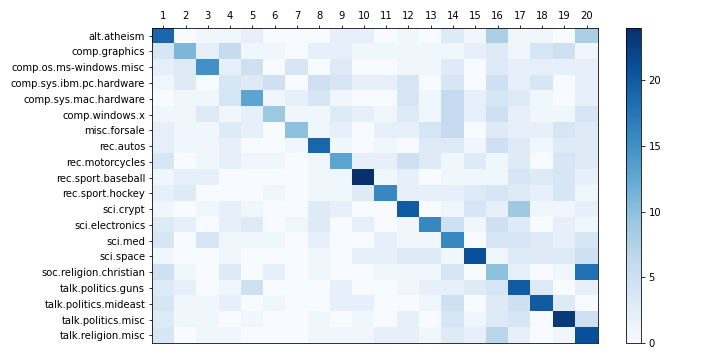
\includegraphics[scale=0.5]{figures/classification_d=50.png}
      \caption{Classification Accuracy. Each square (A,B) is a count of the number of articles in A whose nearest neigbor is in group B. This is for $d=50$}
      \label{fig:classification_d_50}
    \end{figure}
    \begin{figure}[!ht]
      \centering
      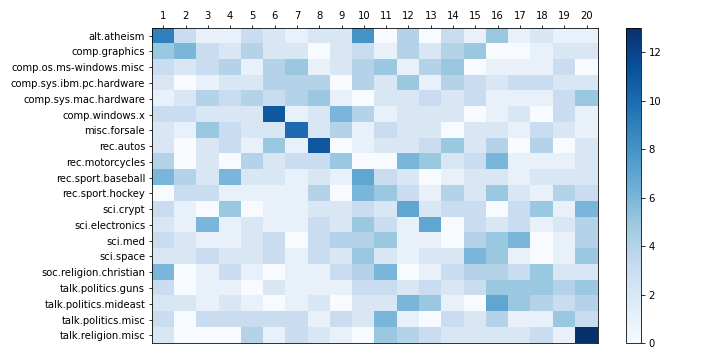
\includegraphics[scale=0.5]{figures/classification_d=100.png}
      \caption{Classification Accuracy. Each square (A,B) is a count of the number of articles in A whose nearest neigbor is in group B. This is for $d=100$}
      \label{fig:classification_d_100}
    \end{figure}

  \item
    We have a dataset with $n$ labeled datapoints, each in $\mathbb{R}^k$. The reduced dimension is $d$.

    The time to reduce the dimensionality of the data is simply the time it takees to multiple an $(nxk)$ matrix with a $(k, d)$ matrix. As such, using naive matrix multiplication, the running time is $O(nkd)$.

    The running time to classify a new article is given by first project this article into $d$ space, which takes $O(kd)$ time. Computing the cosine/jaccard/l2 similarity against a single element in our database takes $O(d)$ time, which we must repeat for all $n$ labeled points. The total runtime is then $O(nd)$, giving a final running time of $O(d(n + k))$.


    In the case where we know that our dataset will be relatively sparse (eg, only 50 words are used in a given tweet), we can make use of $kd$-trees to speed up the search time without needing to reduce the dimensionality at all. This is because when we're checking the extrema of our bounded node in the kd-tree, we will need to look only at $d=50$ dimensions in the worst case (all other will not matter for our datapoint) when using the cosine similarity metric. This reduces our query time to simply the time it takes to search the kd-tree, which has depth $\log n$. Since our dimension is bounded by 50, we will look in at most $O(2^{\sqrt{d}})$ sub-trees, meaning the total runtime will be $O(2^{\sqrt{d}} \log n)$.

    Compared to the system which first reduces the dimensionality, this runtime is significantly faster. The runtime of the reduced dimensionality system is $O(d(n + k))$. For $d = 50$, the runtime comparisons are $O(2^{\sqrt{50}} \log n) = 134*O(\log n)$ wherease the reduced dimensionality system will have runtime of $O(50(n + k))$. For extremely large $n$, the kd tree approach will be much better.
\end{enumerate}


\newpage
\section*{Part 3}

\begin{enumerate}[label=(\alph*)]
  \item
    We consider the $i$-th hash tables in the above scheme, corresponding to matrix $M_i$. For two vectors, $x,y \in R^{k}$ that form an angle of $angle(x,y) = \theta < \frac{\pi}{2}$ radians (i.e.$x$ and $y$ form an acute angle of $\theta$).

    We seek to calculate the probability that $x$ and $y$ hash to the same bucket. We claim the following:
    \[
      \Pr[\text{sgn}(M_ix) == \text{sgn}(M_iy)] = \left(1 -\frac{\theta}{\pi}\right)^{2^d}
    \]
    To see why, we first note that the probability can be broken up into each dimension. That is to say:
    \begin{align*}
      \Pr[\text{sgn}(M_ix) == \text{sgn}(M_iy)] &= \prod_{j=1}^{2^d} \Pr[\text{sign}(m_d x) == \text{sign}(m_dx)] \tag{All coordinates need to have the same sign} \\
      &= \left[\Pr[\text{sign}(m_d x) == \text{sign}(m_dx)]\right]^{2^d} \tag{Each $m_d$ is iid}
    \end{align*}
    As such, we can focus on the inner term, which is just asking what the probability is of the sign for a single coodirnate matching. Recalling that the sign of the inner product between two vectors will be positive if and only if the angle formed between then is less than $\frac{\pi}{2}$ (acute), the inner probability above is precisely given by the probability that a random vector will form an acute angle with both of the vectors $x$ and $y$. If the angle between the vectors $x$ and $y$ is $\theta$, this probability precisely given by (note that the obture case is just a mirrow of this, so it doesn't affect the probability):
    \[
      \frac{(\pi - \theta)}{\pi}
    \]
    Simplifying, this gives us $1 - \frac{\theta}{\pi}$. As some quick spot checks, if $\theta = \frac{\pi}{2}$, the random vector must fall between the two vectors, which will occur half of the time. If $\theta = 0$, it doesn't matter what the random vector is, the signs will always match. 

  \item
    Following the same log as in (a), the probability is given by the likelihood that the randomly chosen vector form an acute angle (or the mirror) with both $x$ and $y$, and since these are separated by at least $2\theta$, then the probability is given by at most:
    \[
       \Pr[\text{sgn}(M_ix) == \text{sgn}(M_iy)] \leq \left(1 - \frac{2\theta}{\pi} \right)^{2^d}
    \]

  \item
    We now consider an applied case where we have a dataset consisting of $n = 1,000,000$ points. We claim that we should choose the values $l = 10,000$ and $d = 8$, and that this satisfies the requirements stated for our specific problem .

    We tackle each requirement in turn to demonstrate that they are all satisfied.

    \begin{itemize}
      \item The first requirement is that we need to correctly identify the nearest neighbor with at least probability of $0.9$ (we succeed at least 9 out of 10 times). Let $x_i$ be the appropriate nearest neigbor where we know that $angle(x_i, y) \leq 0.1$ radians. Then by (a), for a single hash table $j$, the probability of collision is precisely at least:
      \[
        \Pr[\text{sgn}(M_jx_i) == \text{sgn}(M_jy)] \geq \left(1 -\frac{0.1}{\pi}\right)^{2^d} = 0.968169^{2^d}
      \]
      This means the probability of not colliding is at most:
      \[
        \Pr[\text{sgn}(M_jx_i) \neq \text{sgn}(M_jy)] \leq 1 - \left(1 -\frac{0.1}{\pi}\right)^{2^d} = 1 - 0.968169^d
      \]
      If we have $l$ hash tables, then probability that none of them collide (eg, that we do not identify the correct nearest neighbor), is at most:
      \[
          \Pr[\text{sgn}(M_jx_i) \neq \text{sgn}(M_jy), \forall j] \leq \left[1 - \left(1 -\frac{0.1}{\pi}\right)^{2^d}\right]^l = \left[1 - 0.968169^{2^d}\right]^l
      \]
      As such, the probability that we do successfully collide for at least one of our $l$ hash tables is at least:
      \[
        \Pr[\exists j, \text{ st. } \text{sgn}(M_jx_i) == \text{sgn}(M_jy)] \geq 1 -  \left[1 - \left(1 -\frac{0.1}{\pi}\right)^{2^d}\right]^l = 1 -\left[1 - 0.968169^{2^d}\right]^l
      \]
      Looking at the above, we note that larger values of $d$ lead to smaller lower bounds (and that the function is very sensitive to $d$), and larger values of $l$ lead to higher lower bounds. As such, intuitively we can trade these two parameters off to achive our desired lower bound of $0.9$. In fact, for our chose of $l$ and $d$, we have:
      \[
        \Pr[\exists j, \text{ st. } \text{sgn}(M_jx_i) == \text{sgn}(M_jy)] \geq 1 -  \left[1 - \left(1 -\frac{0.1}{\pi}\right)^{2^d}\right]^l = 0.920543
      \]
    \item
      The second requirement is that we don't have too many false positives (eg, we don't have too many values that are incorrectly considered during our search). If we only cared about the first requirement, we could trivially make $d = 1$ and $l$ extremely large, but as we will see, this will need to many false positives.

      More precisely, what we wish to do is place an upperbound on the probability that an element $x_i$ where $angle(x_i, y) > 0.2$ will hash to at least one bucket. Then we will seek to make this upperbound small.

      Following a very similar logic to that presented above, we have that:
      \[
        \Pr[\exists j, \text{ st. } \text{sgn}(M_jx_i) == \text{sgn}(M_jy)] < 1 -  \left[1 - \left(1 -\frac{0.2}{\pi}\right)^{2^d}\right]^l = 1 - \left[ 1 - 0.936338^{2^d} \right]^l
      \]
      With this probability, we have that in expectation the number of elements our algithm will consider will be the $1$ (the true element) plus the elements in $(0.1, 0.2)$ (which by assumption is ``not too many'') plus:
      \[
        n\left(1 -  \left[1 - \left(1 -\frac{0.2}{\pi}\right)^{2^d}\right]^l \right)
      \]
      Obviously, the natural tradeoff here is that the expectation is small the smaller $l$ is and the larger $d$ is. In a sense, this requirement is in exact opposition to the previous requirement, which means we need to find a subtle balance between the two in order to achive our goal.

      In fact, wiht our values of $n, l$ and $d$, we have:
      \[
        1000000\left(1 -  \left[1 - \left(1 -\frac{0.2}{\pi}\right)^{2^d}\right]^l \right) = 486.021
      \]
      Which means in expectation we'll have a low number of unnecessarily collisions.

    \item
      For the last requirement, we just need to make sure that the running time to compute all $l$ hashes is small. This requirement implies that we want both $d$ and $l$ small, since the total running time is roughly $O(ld)$ (we compute $l$ hashes, and each hash requires a dot product over $d$ dimensions).

      The above setup satisfies this requirement. The run-time will be dominated by the expected number of collinding elements, which we've kept to ~1000. Similarly, the number of hashes has been kept to ~10,000, which means overall running time will be in the order of 20,000 operations rather than 1,000,000 * k as before. This seems like a reasonable tradeoff.
    \end{itemize}

  \item
    Code used for this section is presented below:
\begin{verbatim}
class RandomHyperplaneClassifier:
    def __init__(self, d: int, k: int, l: int):
        """Initializes the RandomHyperplaneHasher.

        Given a vector x \in R^k, the for each hash table we compute
        hash = bucket(Mx) where M is drawn uniformly at random (but fixed)
        for each hash table and bucket returns the corresponding digit in
        [0, 2^d-1].

        Args:
            l: The number of hash tables to construct.
            d: Each hash table will have 2^d buckets.
        """
        # Each hash table points to a list of tuples of (articleIdx, article) that
        # hashed to that bucket.
        self.d = d
        self.l = l
        self.k = k
        self.hash_tables = [{} for _ in range(l)]
        self.hash_matrices = [
            scipy.sparse.csr_matrix(np.random.normal(size=(d, k)))
            for _ in range(l)]
        self._powerMatrix = np.array([2**i for i in range(d)]).reshape((1, d))
        self._db = None
        
    def _hash(self, db):
        """Computes the l hash values of all provided elements.
        
        Args:
            db: (n, k) matrix of n elements to be hashed.
            
        Returns:
            A list of l numpy arrays of shape [n] specifying the indexes
            for each of the n elements into the l-th hash table.
        """
        hashes = []
        n, _ = db.shape
        for i, M in enumerate(self.hash_matrices):
            P = np.dot(db, M.T).todense() # (n,d)
            n, d = P.shape
            P[P > 0] = 1
            P[P <= 0] = 0
            indices = np.array(np.sum(
                np.multiply(P,  self._powerMatrix), axis=1)).flatten().astype(int)
            hashes.append(indices)
        return hashes
    
    def _load(self):
        """Computes the load of each hash table. Load is defined as average number of elements per bucket."""
        return [np.mean([len(els) for els in table.values()]) * len(table) / 2**self.d
                for table in self.hash_tables]
    
    def add(self, db):
        """Adds the given set of elements to the hasher. Should only be called once.
        
        Args:
            db: An (nxk) sparse matrix where each row corresponds to an element
                to be added to the hasher.
        """
        assert not self._db
        print("Adding elements for d=%s, l=%s" % (self.d, self.l))
        all_hashes = self._hash(db)
        for m, element_hashes in enumerate(all_hashes):
            table = self.hash_tables[m]
            for row_idx, element_hash in enumerate(element_hashes):
                if element_hash in table:
                    table[element_hash].append((row_idx + 1, db.getrow(row_idx)))
                else:
                    table[element_hash] = [(row_idx + 1, db.getrow(row_idx))]
        self._db = db
        print("Added elements for d=%s, l=%s" % (self.d, self.l))
        return True
                
    def neighbors(self, db):
        """Classifies the elements.
        
        Args:
            db: A matrix [n,k] of n elements to classify.
        
        Returns:
            A list of n integers specifying the articleIdx of the closest neighbor.
        """
        print("Getting neighbors elements for d=%s, l=%s" % (self.d, self.l))
        all_hashes = self._hash(db)
        n, _ = db.shape
        sq = [[] for i in range(n)] # List of sq for each datapoint.
        sq_indexes = [[] for _ in range(n)] # Each inner list maps sq[i][j] to sq_indexes[i][j].
        sq_sets = [set() for _ in range(n)] # Each inner list is a set of the unique elements included in sq_indexes[i][j]
        our_document_idx = [] # Gives us the idx in sq* that corresponds to our document.
        for m, element_hashes in enumerate(all_hashes):
            table = self.hash_tables[m]
            for row_idx, element_hash in enumerate(element_hashes):
                if element_hash in table:
                    for articleIdx, article in self.hash_tables[m][element_hash]:
                        if articleIdx not in sq_sets[row_idx]:
                            sq_sets[row_idx].add(articleIdx)
                            sq[row_idx].append(article)
                            sq_indexes[row_idx].append(articleIdx)
                            if (row_idx + 1) == articleIdx:
                                our_document_idx.append(len(sq[row_idx]) - 1)
        
        sq_matrices = [scipy.sparse.vstack(sqs) for sqs in sq]
        average_size = np.mean([len(sqs) for sqs in sq])
        print("Average size of SQ is %s for d=%s, l=%s, k=%s" %(average_size, self.d, self.l, self.k))
        
        # Create sparse matrices.
        nearest_neighbors = []
        for our_doc, sq_matrix, sq_index in zip(our_document_idx, sq_matrices, sq_indexes):
            idxes = find_nearest_neighbor(sq_matrix, cosine_dist) - 1 # (#sq, #sq)
            # Our document is the first row, map back to full databses.
            neighbor_idx = sq_index[idxes[our_doc]]
            nearest_neighbors.append(neighbor_idx)
        
        print("Got neighbors elements for d=%s, l=%s" % (self.d, self.l))
        

        return np.array(nearest_neighbors), average_size

def problem3d():
    l = 128
    data = read_data()
    n, k = data[0].shape
    sizes = []
    accuracies = []
    for d in range(5, 21):
        avg_size = None
        def nn(db, sim_fn):
            hasher = RandomHyperplaneClassifier(d=d, l=128, k=k)
            hasher.add(db)
            nns, avg_size = hasher.neighbors(db)
            return nns

        accuracy = plotHeatMaps2(*data, figName='local_sensitivity_hashing_l=%s_d=%s' % (l, d),
                                 nearest_neigbor_fn=nn)
        sizes.append(avg_size)
        accuracies.append(accuracy)
    return sizes, accuracies

\end{verbatim}

    Plotting classification accuracy versus the average size of the $S_q$ set, we see the results in Figure \ref{fig:accuracy_as_sq}, As we can see below, there does appear to be a sweet spot in the classification where the accuracy does not decrease significantly but we can reduce the size of our $S_q$ set to ~200 elements, rather than 1000.

    \begin{figure}[!ht]
      \centering
      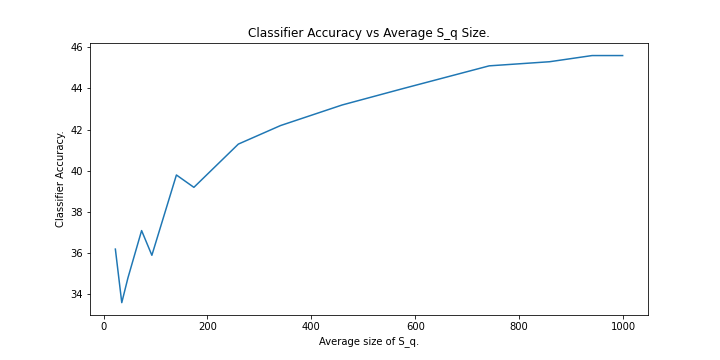
\includegraphics[scale=0.5]{figures/Classifier_vs_s_q_size.png}
      \caption{Accuracy as a Function of $S_q$}
      \label{fig:accuracy_as_sq}
    \end{figure}

    The resulting accuracies and sizes are:

    Average size of SQ is 999.172 for d=5, l=128, k=61067

    Average size of SQ is 987.826 for d=6, l=128, k=61067

    Average size of SQ is 940.396 for d=7, l=128, k=61067

    Average size of SQ is 858.53 for d=8, l=128, k=61067

    Average size of SQ is 742.308 for d=9, l=128, k=61067

    Average size of SQ is 576.98 for d=10, l=128, k=61067

    Average size of SQ is 459.338 for d=11, l=128, k=61067

    Average size of SQ is 340.664 for d=12, l=128, k=61067

    Average size of SQ is 259.502 for d=13, l=128, k=61067

    Average size of SQ is 173.936 for d=14, l=128, k=61067

    Average size of SQ is 140.306 for d=15, l=128, k=61067
    
    Average size of SQ is 93.07 for d=16, l=128, k=61067
    
    Average size of SQ is 73.304 for d=17, l=128, k=61067
    
    Average size of SQ is 46.978 for d=18, l=128, k=61067
    
    Average size of SQ is 35.128 for d=19, l=128, k=61067
    
    Average size of SQ is 22.802 for d=20, l=128, k=61067
    

    Classification accuracy: 45.60\% for local\_sensitivity\_hashing\_l=128\_d=5

    Classification accuracy: 45.60\% for local\_sensitivity\_hashing\_l=128\_d=6

    Classification accuracy: 45.60\% for local\_sensitivity\_hashing\_l=128\_d=7

    Classification accuracy: 45.30\% for local\_sensitivity\_hashing\_l=128\_d=8

    Classification accuracy: 45.10\% for local\_sensitivity\_hashing\_l=128\_d=9

    Classification accuracy: 44.00\% for local\_sensitivity\_hashing\_l=128\_d=10

    Classification accuracy: 43.20\% for local\_sensitivity\_hashing\_l=128\_d=11

    Classification accuracy: 42.20\% for local\_sensitivity\_hashing\_l=128\_d=12

    Classification accuracy: 41.30\% for local\_sensitivity\_hashing\_l=128\_d=13
    
    Classification accuracy: 39.20\% for local\_sensitivity\_hashing\_l=128\_d=14
    
    Classification accuracy: 39.80\% for local\_sensitivity\_hashing\_l=128\_d=15
    
    Classification accuracy: 35.90\% for local\_sensitivity\_hashing\_l=128\_d=16
    
    Classification accuracy: 37.10\% for local\_sensitivity\_hashing\_l=128\_d=17
    
    Classification accuracy: 34.80\% for local\_sensitivity\_hashing\_l=128\_d=18
    
    Classification accuracy: 33.60\% for local\_sensitivity\_hashing\_l=128\_d=19
    
    Classification accuracy: 36.20\% for local\_sensitivity\_hashing\_l=128\_d=20


    We include all the relevant heatmaps as well.
    \begin{figure}[!ht]
      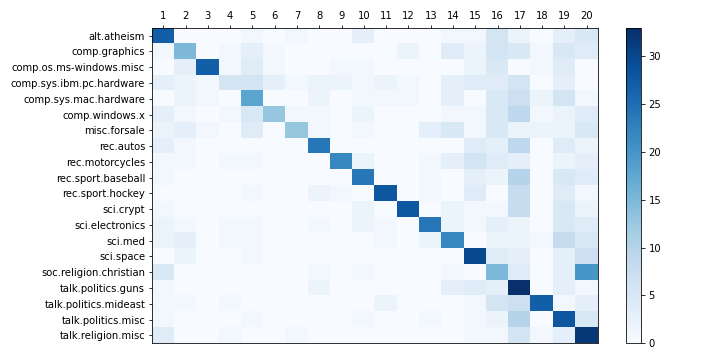
\includegraphics[scale=0.2]{figures/local_sensitivity_hashing_l=128_d=5.png}
      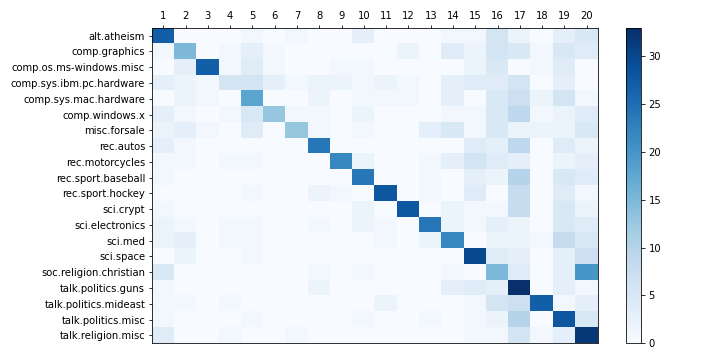
\includegraphics[scale=0.2]{figures/local_sensitivity_hashing_l=128_d=6.png}
      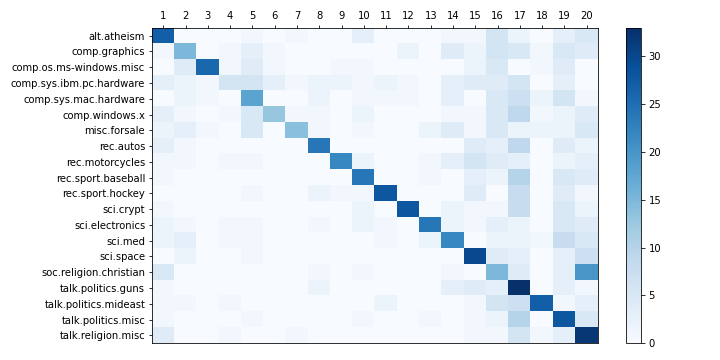
\includegraphics[scale=0.2]{figures/local_sensitivity_hashing_l=128_d=7.png}
      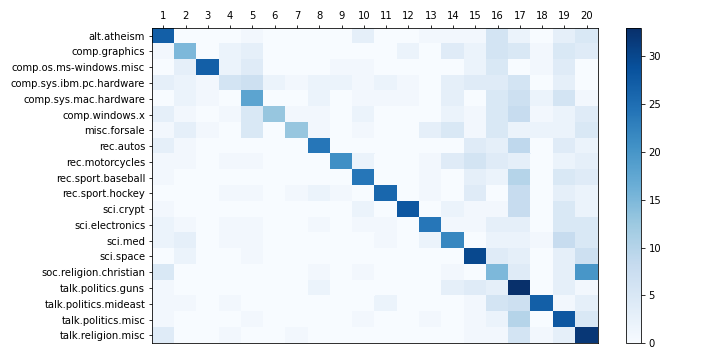
\includegraphics[scale=0.2]{figures/local_sensitivity_hashing_l=128_d=8.png}
      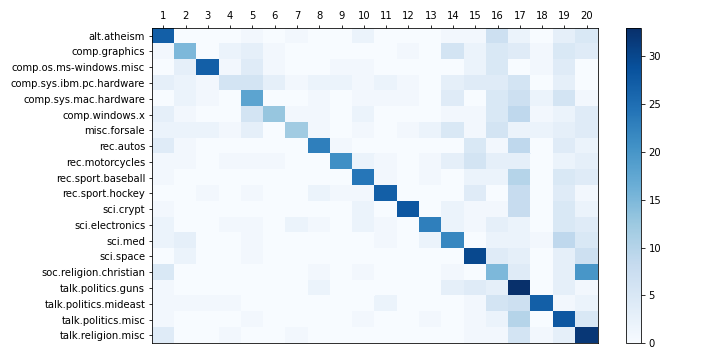
\includegraphics[scale=0.2]{figures/local_sensitivity_hashing_l=128_d=9.png}
      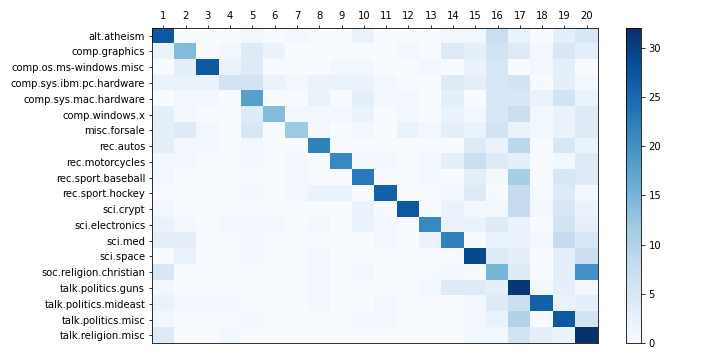
\includegraphics[scale=0.2]{figures/local_sensitivity_hashing_l=128_d=10.png}
      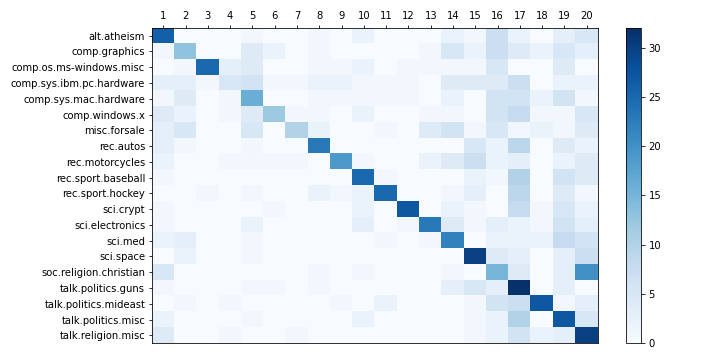
\includegraphics[scale=0.2]{figures/local_sensitivity_hashing_l=128_d=11.png}
      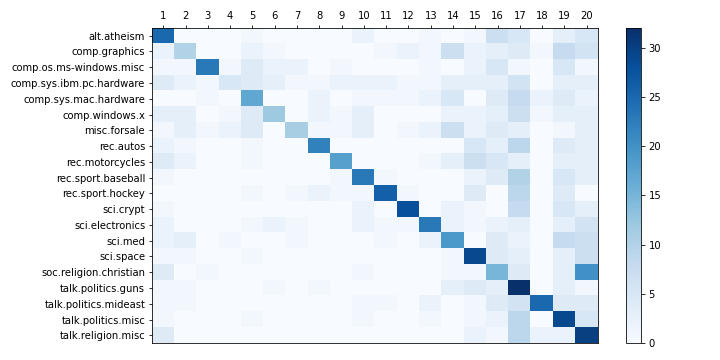
\includegraphics[scale=0.2]{figures/local_sensitivity_hashing_l=128_d=12.png}
      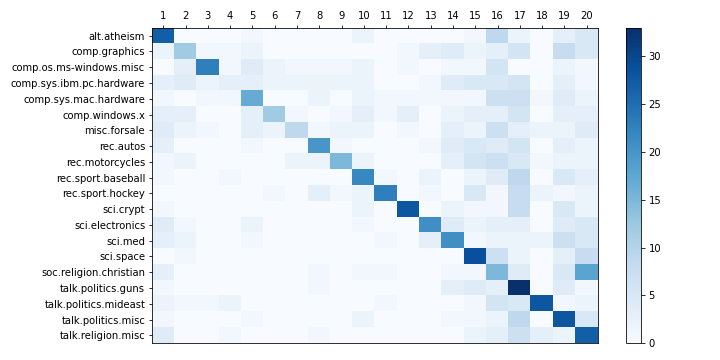
\includegraphics[scale=0.2]{figures/local_sensitivity_hashing_l=128_d=13.png}
      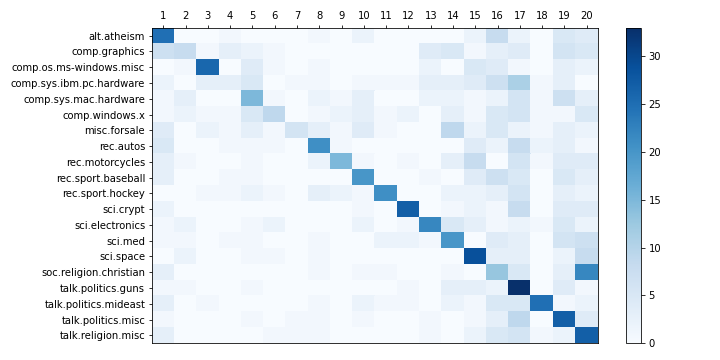
\includegraphics[scale=0.2]{figures/local_sensitivity_hashing_l=128_d=14.png}
      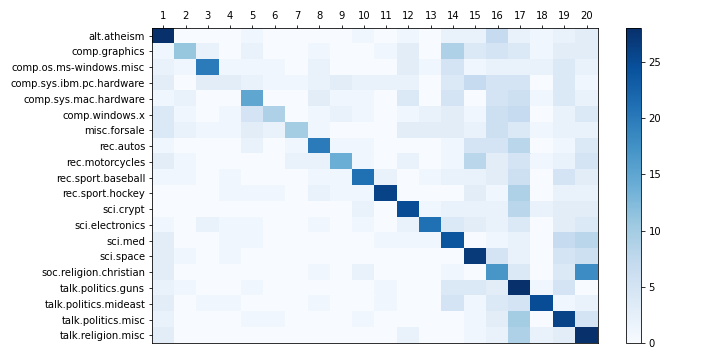
\includegraphics[scale=0.2]{figures/local_sensitivity_hashing_l=128_d=15.png}
      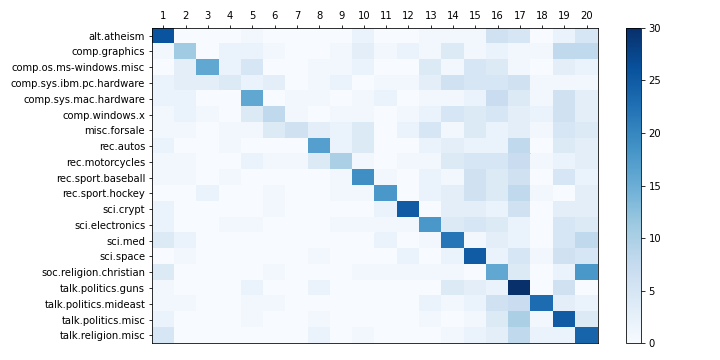
\includegraphics[scale=0.2]{figures/local_sensitivity_hashing_l=128_d=16.png}
      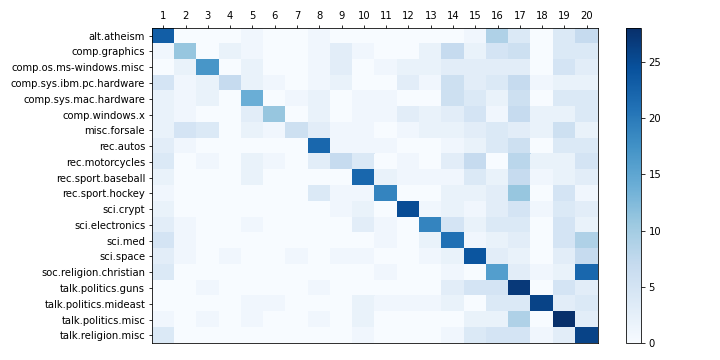
\includegraphics[scale=0.2]{figures/local_sensitivity_hashing_l=128_d=17.png}
      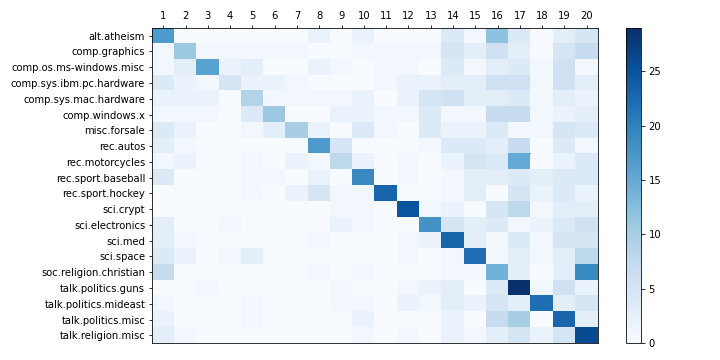
\includegraphics[scale=0.2]{figures/local_sensitivity_hashing_l=128_d=18.png}
      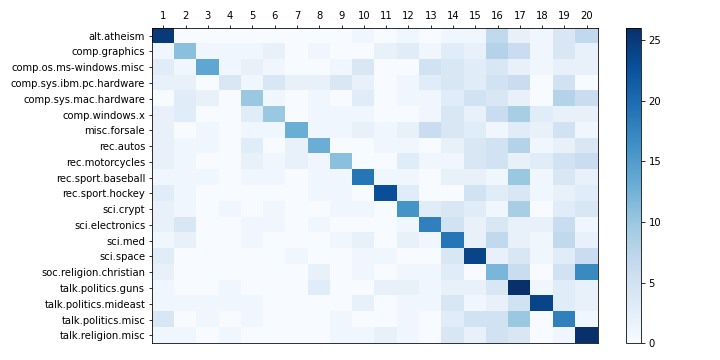
\includegraphics[scale=0.2]{figures/local_sensitivity_hashing_l=128_d=19.png}
      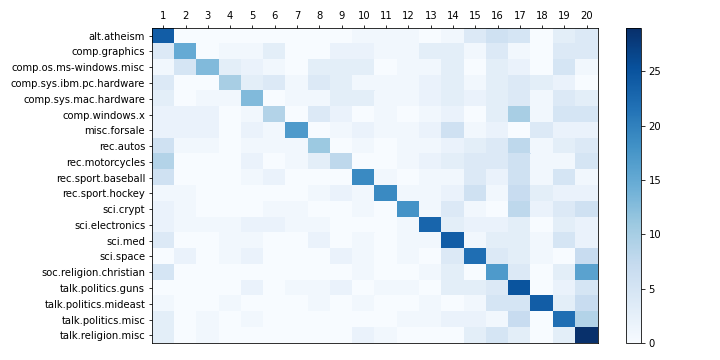
\includegraphics[scale=0.2]{figures/local_sensitivity_hashing_l=128_d=20.png}
      \caption{Relevant heatmaps. Ordered left-to-right and top-to-bottom from $d=5$ to $d=20$ with $l=128$ for all of them.}
    \end{figure}

  \item
    The LSH-based classification system achieves good performance with a sufficient number of hash functions and buckets. The optimal dimensionality required $d$ is significantly smaller than that required by the dimension-reduction-based (DRB) system in Problem 2. However, it does require significantly more hash functions, which can make it costly during inference, and is something not required by the DRB system. Another interesting point to draw is that the DRB system requires less storage (since we store a heavily compressed version of the data). However, the LSH-based system always stored the original dataset, and without optimizations, can even store duplicate copies of the original.

    Given these properties, a system that is light on memory would likely benefit from the DRB system since it not only improves performance but also generally reduces the cost of storage. However, a system where storage constraints are not that important and which is instead more interested in latency would benefit from the LSH-based system, since the number of elements we compare to can be relatively small with only the cost of a few hash functions.

    The memory aspect also leads to some discussion of how the two systems could be combined. Given that the random project statistically preserves angles, we could combine the systems by first projecting our original datapoints into a lower dimension, and storing these in the LSH-based system. When we do the brute-force search over $S_q$, we would take advantage of this and compare projections to projections. This should further speed up the brute-force search.
\end{enumerate}

\newpage
\section*{Appendix}
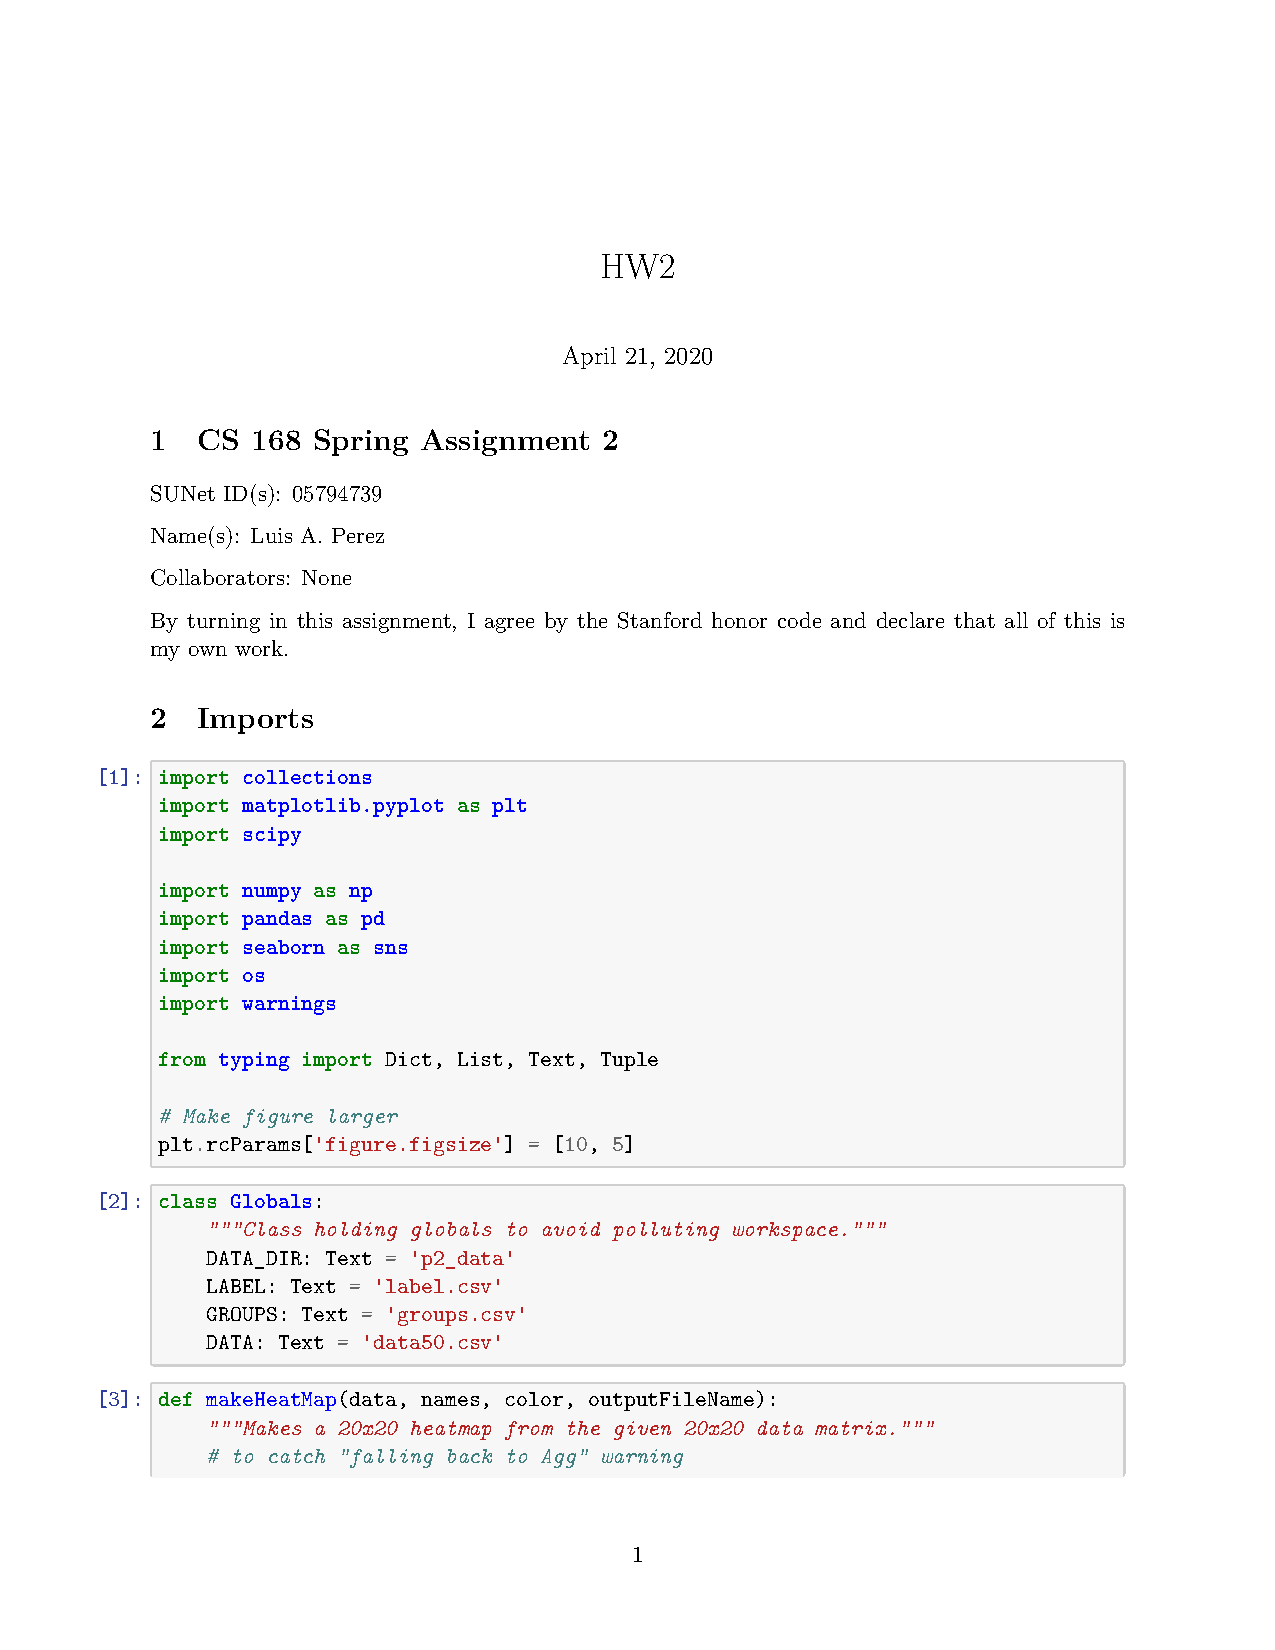
\includepdf[pages=-]{HW2}

\end{document}
